\chapter{Big Data Architecture}
\label{chap:big_data_architecture}

Traditionally, the process of making decisions is expensive and experiences significant error.
Simple reasoning is a straightforward approach, but it can work only till the certain point.
The main problem is that it can be easily ruined by the wrong assumptions.
Hence one would preferably use evidence based approaches that built on the accumulated data.
The most commonly used tools for this purpose are surveys and experiments, carried out on a control group.   
However, they both have significant disadvantages that makes the process of making decisions more complicated. 
On the one hand, surveys and experiments involve human resources, what leads to high expenses.
On the other hand, these approaches are also vulnerable to errors.
A lot of various reasons can cause an error, such as a survey composed in a wrong way, or a not representative control group.
 
Fortunately, this situation has changed dramatically in recent years.
First of all, data has become available for free, as a by-product of other processes (such as log files).
Moreover, constant reduction of data storage costs allows to warehouse enormous amounts of information, without troubling about the size limits.
Owing to the progress in the information technologies area, both transferring and processing of huge data volumes become easy.
All this gives us an alternative solution to the problem of making decisions that avoids the drawbacks of the strategies presented above.
The name of this solution is Big Data.

The main distinguishing feature of Big Data is that data collection is independent of use case.
Information is collected because it is available and cheap, with the hope that later on it can be used to answer a question that has not arisen yet.
For example, Facebook stores all available data about the users, like demographic information, geographic location, connections with other users, visited websites, clicked links, etc.
As a result it has a huge amount of data, which, with the right approach, can give lots of useful information. 
For instance, afterwards it can be used in targeted advertising, or for performing the social network analysis.

\authorsection{Big Data}{SP}
\mnote{Big Data}
There is no consensus about the origins of the term "Big Data", but most of the sources claim that it is first mentioned in the press in 2008.
People start actively using it since 2009 and it spreads quickly owing to its precise and capacious meaning. 
Big Data is characterized by its high (i) variety, (ii) velocity and (iii) volume. [reference]

\mnote{variety}
First, Big Data sources are highly diverse.
They differ in the type of produced data - it can be text, images, sounds, raw feed incoming directly from sensors, etc.
Each of these types, in turn, may have a different format.
For instance, text can be transmitted in various languages, coding, formatting and so forth.
Big Data sources also differ in the speed of data flow and the data purity.  
Some of the sources generate noisy information, while others can produce data, that does not need cleaning.
On the other hand, Big Data differ in the way how it is collected, how urgently it should be processed and which storage capabilities are available for its warehousing.

\mnote{velocity}
The diversity of Big Data sources causes the high velocity of data input flow.
For example, [Menthal]
Since data arrives at a high speed, there is a high chance that the velocity of its transmission and processing should also be high.
For instance, it can help to improve traffic in metropolitan areas, offering various travel alternatives for a vehicle, basing on analysis of incoming data about the situation on the roads.
Rapidity of data processing can be necessary in other cases as well.
Sometimes high processing speed can even be indispensable to life, when using in medicine, for example.
Special systems monitor the state of a patient, immediately alerting caregivers in the case of dangerous anomaly occurrence. 

\mnote{volume}
In the end, massive sources variety, multiplied by high velocity of data generation, results in its enormous size.
For instance, by the end of 2013, the number of Facebook users reaches 1.23 billion.
Each of them not only has some profile information, but also communicates with other users, shares data, updates the timeline and so forth.
In total 2.5 billion content items are shared every day.
Let us assume that each of these events is stored as a JSON object and needs 2Kb on average.
That means that in the end of the year Google deals with 4.65Tb * 365 = 1.65Pb of information.
And it is only metadata, not including images and video files that require significantly more space. 
As a result, Facebook deals with storing and processing petabytes of data.

Another example is the information received from sensors.
Sensor is a converter that measures and transforms physical quantity into a digital signal.
Sensors find an application in various fields: manufacturing industry, transportation systems, meteorology, medicine, even modern smartphones have lots of sensors.
The key feature of a sensor is that often it does its job constantly, continuously producing the flow of information, what leads to the large volumes of data.
Nest Labs is an American company that manufactures sensor-driven thermostats and smoke detectors.
The population of United States is about 318 million, so if every hundredth resident uses at least one of Nest thermostats in the house, it sums up to 3.2 million devices.
One thermostat has a variety of sensors, like activity, temperature, humidity, illumination, etc.
They generate and transmit around 2Mb of data per day, or, consequently, 2.17Tb per year. 
The ability to process large amounts of information is the main benefit of Big Data analytics, since with its vast volume it is possible to construct better models.
All these three "v": volume, velocity and variety constitute a criterion that allocates Big Data observation into a distinct sector of computer science, which requires ad hoc decisions and a special approach.

\mnote{Batch processing}
There are two fundamentally different ways of processing the Big Data, namely Batch and Real Time data processing.
In the first case, data is handled in batches, i.e. process collects the data until the batch size is obtained, and only after this the process can perform the necessary actions on a batch as a whole.
This gives several advantages.
Obviously, it becomes possible to process multiple operations in one request, instead of handling each operation individually.
That makes data treatment more efficient. 
To give a naive example how batching improves the performance, let us describe the problem of I/O operations.
I/O operations involve physical movement of mechanical devices (e.g. seek motion of hard drive).
Thus, the speed of sequential writes to a file is higher than random writes, because in the latter case additional time is spent for seek operations between each write.   
Batch processing can be done in the appropriate time, when the computing resources are less busy.
Furthermore, one can set a priority for each task, beginning with more urgent operations.
There is no need in a close supervision of a run, batch processing is mostly autonomous.
However, there is a significant drawback.
The results are always obtained with an arbitrary time delay.

\mnote{Real Time processing}
Real time processing handles data at the moment of arrival. 
The advantage of the latter is that the results are ready almost immediately, which can be an essential requirement in such areas as medicine or security threat prediction. 
In spite of the fact that a certain delay is nevertheless exists, its duration is predetermine and is guaranteed to have a specified value.
That differentiates real time processing from batch processing.
This fixed delay length varies depending on the application.
In some cases 10 minutes to perform all the computations is still considered to be a real time processing.
However, in other cases, more than 1 second delay is unacceptable.
Real time processing makes the information always available and up-to-date.
These significant advantages results in rising popularity of real time processing, despite the fact that it requires greater effort to design and maintain.

\authorsection{Architectural Requirements}{SP}
Big Data technology is an umbrella of various systems. 
Data has to be collected, processed, transmitted, stored, protected from attacks, etc.
The [Figure 3.1] shows the general flow of data within the Big Data concept.
Each of the presented steps involves a batch of technologies.
For example, depending on data type and size, one can choose SQL (MySQL, Oracle, Teradata, etc.) or NoSQL (Cassandra, MongoDB, Apache HBase, etc.) solutions for storing Big Data.
Similarly, depending on the application, Real Time processing (Storm, Spark Streaming, etc.) or Batch processing (Apache Hadoop, etc.) technologies are used. 
Thereby, it is apparent that no one general solution exists for every Big Data problem.

\begin{figure}
  \centering
  \includegraphics [width=0.9\textwidth]{images/big_data_flow}
  \caption{Big Data Flow}
  \label{Fig.3.1:Big Data Flow}
\end{figure}

Well thought-out structure of Big Data architecture is of big importance.
As it follows from the previous paragraph, Big Data architectures have to be targeted to each specific scenario.
For instance, architecture, designed for processing video data from a web camera, differs significantly from one for handling server log files.
Menthal, [Menthal: definition] mentioned above, deals with data, that consists of a bulk of small text messages(?). 
In the following sections we describe the existing Big Data architectures in the context of Menthal needs.

It is natural to start with a naive approach, using widely available and easy to use technologies.
[Menthal: MySQL + what else?]
However, at a certain point, a naive approach cannot anymore sustain a constantly growing load.
Hence the biggest IT corporations conduct their own research in this area, designing specific architectural solutions for working with Big Data.

\mnote{Google architecture}
Google is one of the well-known examples of such corporations.
Its activity directly relates to storing and processing of Big Data.
Google Search engine handles more than three billion searches every day.
Social networking service Google+ had 540 million users in 2013.
Gmail, Google's email service, had 425 million users in 2012.
These are just several examples of large-scale Google projects, that processes huge amounts of data.
Therefore, Google introduces a batch of solutions for building scalable systems. 

The overall structure of Google Big Data architecture is presented in [Figure 3.2].
The lowest layer is Google File System - scalable and highly available file system. 
These properties are achieved by replicating data across several machines.
Next, data can be efficiently processed by MapReduce framework.
This technology includes two steps - map, that performs filtering and sorting and reduce, that aggregates the output of map step to the final result.
Bigtable, a highly scalable database, provides a way to store massive amounts of information.
Let us explain in more detail the primary features and internal structure of these technologies.

\begin{figure}
  \centering
  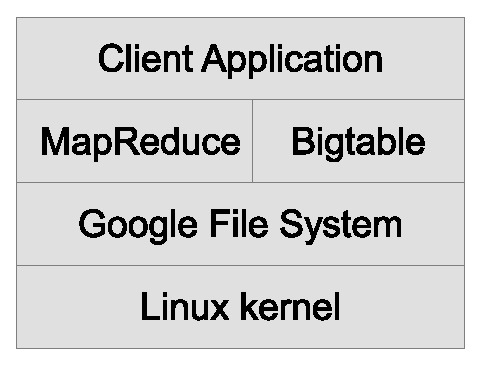
\includegraphics [width=0.9\textwidth]{images/Google_architecture}
  \caption{Big Data Flow}
  \label{Fig.3.1:Big Data Flow}
\end{figure}

\authorsection{Google File System}{SP}
[reference]
\mnote{Google File System}
Google File System (GFS) is a scalable distributed file system, which supports Big Data operations.
The underlying idea is the following: Google Search Engine and some other Google systems process vast amount of data, which is spread all over the world.
Hence the file system should be highly extensible, give an opportunity to use cheap hardware components and, consequently, be fault tolerate. 
Furthermore, it has some specific usage features.
Because of vast scales and cheap hardware, component failure is a commonplace.
The size of files exceeds several-fold the traditional standards, so a multi-gigabyte file is not unusual.
Most of the time the stored data stays unchanged and new data is only appended.
The append operation, in its turn, should provide the concurrent access for multiple clients.

Availability, reliability, scalability and performance are important attributes of a distributed file system.
Availability means that a system operates properly at any given moment.
Reliability denotes the capability of a system to operate continuously without failing.
Scalability indicates the property to handle a growing amount of work.
Performance is a quantitative characteristic of operation speed.  
GFS architecture design helps to meet all these requirements.

[Figure 3.3] illustrates the main components of the GFS Architecture.
Each GFS cluster contains one master server and several chunkservers.
The master has a "shadow" node, that provides read-only access when the primary master is down. 
Chunkserver stores chunks as Linux files on local disk.
Every chunk is replicated on several chunkservers for reliability.
One chunk combines multiple files and has a fixed size of 64 megabytes.

\begin{figure}
  \centering
  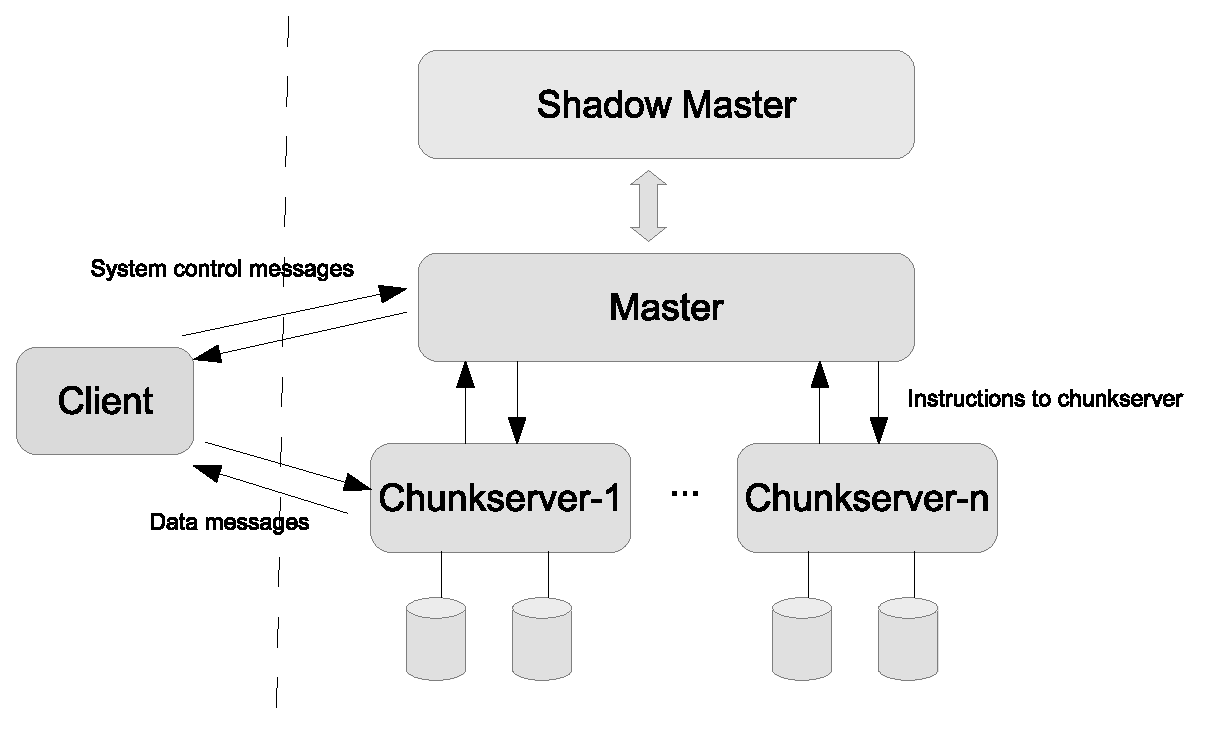
\includegraphics [width=0.9\textwidth]{images/GFS_architecture}
  \caption{Big Data Flow}
  \label{Fig.3.1:Big Data Flow}
\end{figure}

The large size of chunk gives several advantages.
Clients send requests to the master for chunk location less frequently.
A persistent TCP connection to the chunkserver for a longer time period allows to avoid network overhead.
The master node stores less metadata that provide a possibility to keep it in memory.

The master node manages the mapping from files to chunks, location of chunks, access control, garbage collection and some other tasks.
It does not persistently store the information about chunks location. 
On the contrary, it gives instructions to chunkservers and collects their states using periodic HeartBeat messages.
To prevent the master being a bottleneck, only file system control data goes through it.
For example, a client can ask the master node which chunkservers it should contact.
The master node returns the corresponding chunk handle and its replicas' location.
After receiving a reply, the client caches this information and can directly transfer data to the given chunkserver, dispensing master node from overload.
Clients and chunkservers do not cache file data.
Clients mostly work with files that are too large to be cached.
Chunkservers treat chunks as Linux files, therefore in this case caching is done by operating system.

\mnote{operation log}
To recover its state, the master uses the operation log.
The operation log consists of the chronometric information about critical metadata changes.
This log is replicated on several machines.
For the purpose of consistency, client receives a respond for operation only when corresponding log record is flushed to a local disk and the disks of all replicas.
To avoid the operation log being too large, the master makes a checkpoint each time when the log size exceeds a certain threshold.
In the case of failure, the master can load the latest checkpoint from local disk and replay it, recovering its state.
For storing checkpoint it uses a compact B-tree like data structure, that allows to map it directly into memory and perform fast lookups.
For performance reasons the new checkpoint is created in separate thread.
The ability of a server to restore its state does not depend on the way it was terminated.
Shutting down a server by killing the process is a normal procedure. 

\mnote{mutation}
A mutation denotes a change of the contents or metadata of a chunk.
There are two types of mutations, namely writes and record appends.
In the former case data is written with a file offset specified by a client.
In the latter, GFS chooses an offset, and data (record) is appended with an append-at-least-once semantics.
Record append operation is atomic, i.e. it is treated as one continuous sequence of bytes. 
This allows multiple clients to append information concurrently.

\mnote{lease}
Each mutation is replicated across several chunks.
To keep a mutation order consistent at all the replicas, GFS uses a technique of leases.
The master gives a lease to one of the replicas, that becomes a primary replica.
The primary chooses an order for all the chunk's mutations and each replica then follows this order when applying mutations.

The flow of write control is shown on [Figure 3.4] in more details.

\begin{figure}
  \centering
  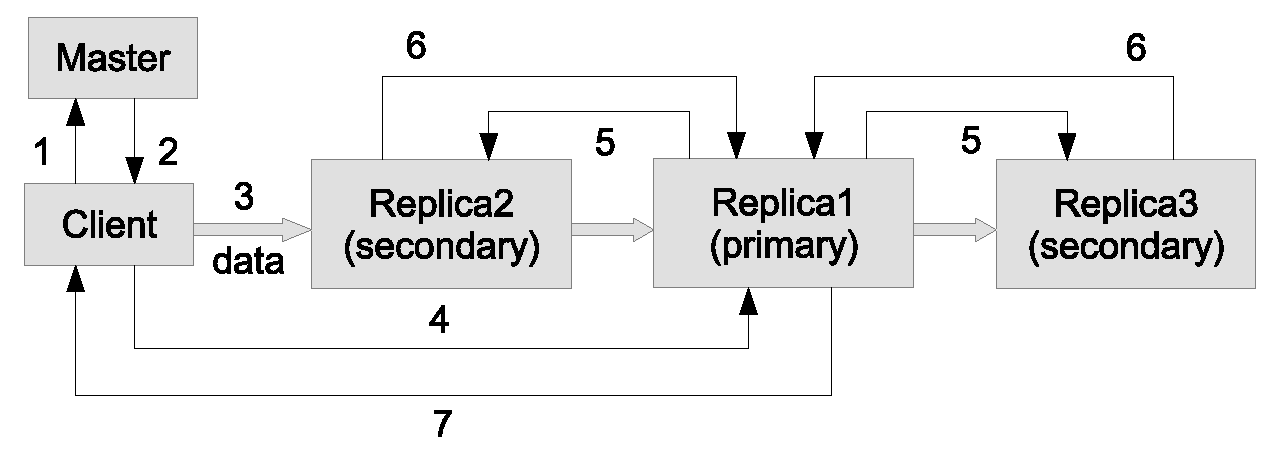
\includegraphics [width=0.9\textwidth]{images/write_control_flow}
  \caption{Big Data Flow}
  \label{Fig.3.1:Big Data Flow}
\end{figure}

1. The client sends a request to the master.
2. The master replies with a chunkserver, that holds the current lease, and the location of the other replicas.
If a primary replica (that has a lease) is not defined, the master chooses one. 
The client caches this information for the next mutations.
3. The client sends the data to all the replicas in arbitrary order.
Chunkservers store this data in an internal buffer cache. 
4. When the client receives acknowledgements from all the replicas, it sends a write request to the primary.
The primary picks serial numbers to all the mutations it has received and performs them in corresponding order.
5. All secondary replicas receive the write request forwarded by the primary.
Each replica applies mutations to its own state in the same order assigned by the primary.
6. The secondaries notify the primary about the completion of the operation.
7. The primary sends a reply to the client.
In the case of error occurrence at any of the replicas, the primary informs the client about them.
The write is considered to be successful, if the primary and an arbitrary number of secondary replicas succeeded.

GFS differs from traditional file systems in the way how it manages files and directories.
There is no possibility to list all the files in a directory in GFS, because it does not support per-directory structure.
It stores a mapping between full pathnames and metadata in a lookup table.
Prefix compression helps to efficiently represent this table in memory. 

The file deletion does not occur at once.
Firstly the master logs the event of deletion.
Than the system renames the file with a hidden name that includes the time of deletion.
The master performs a regular scan of the namespace and removes a hidden file, if it has existed for more than a specified time interval (e.g. 3 days). 

All the described features help the Google File System to successfully cope with a large-scale data processing workload.
GFS meets the storage needs of Google corporation.
Therefore Google uses GFS as the storage platform for many applications, both in research and production areas.
Another Google technologies, like MapReduce or BigTable are based on it.  	 

\authorsection{MapReduce}{SP}
[reference]
MapReduce model finds wide application in a variety of real world tasks.
For example, search engines use web crawling to gather a vast amount of information.
They process this information to create inverted indices, construct web graphs, figure out the most frequent search queries, etc.
Any of these tasks can be divided into two steps, namely Map and Reduce.
Map operation converts input data to a set of intermediate key/value pairs.
Reduce operation, in its turn, combines all the values that share the same key.
The advantage of the MapReduce abstraction is that it hides the implementation details from users.
This allows even not experienced programmers to easily construct parallel and distributed systems.

MapReduce shares the same requirements with other systems that work with large data sets.
It should provide high parallelization, be fault-tolerant and perform load balancing between nodes.
Applying Map and Reduce operations helps to parallelize large calculations.
Moreover, this makes simpler re-execution of a task that serves as a primary mechanism for fault tolerance.

Both Map and Reduce operations work with key/value pairs.
The user of MapReduce library determines the logic of these operations, specific to the given application.
The Map function receives an input key/value pair and produces a set of intermediate pairs.
The MapReduce library groups these intermediate pairs together by the key and passes the result to the Reduce function.
It passes them via iterator that allows to handle a large data set without keeping it in memory.
The Reduce function merges the values with the same key, possibly decreasing a given set of values.
One Reduce function invocation can give only a single output value, or even none.
[Figure 3.5] illustrates a pseudo-code for a simple MapReduce task.

\begin{figure}
  \centering
  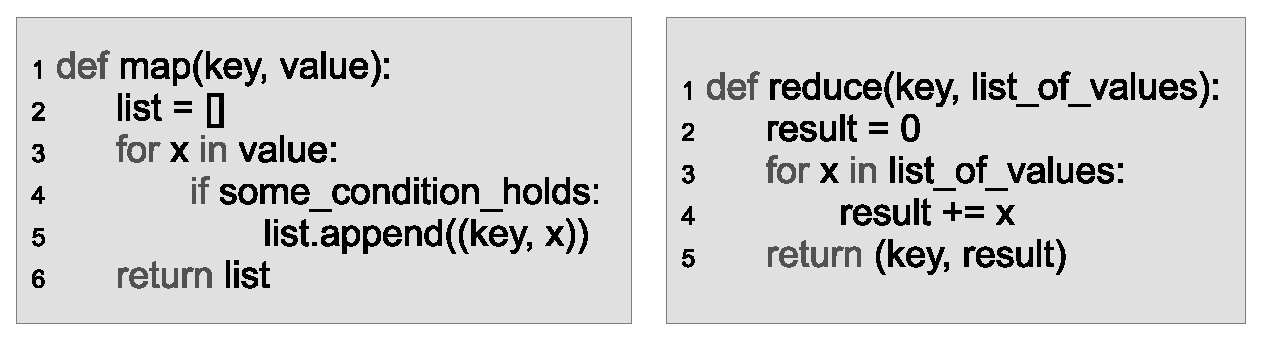
\includegraphics [width=0.9\textwidth]{images/MapReduce_pseudo_code}
  \caption{Big Data Flow}
  \label{Fig.3.1:Big Data Flow}
\end{figure}

We visualize the overall flow of a MapReduce operation in [Figure 3.6].
1. The MapReduce library divides the input files into M splits.
The size of one piece varies from 16Mb to 64Mb depending on the chosen settings.
User code invokes the MapReduce routine on several machines.
2. One of these machines is a master, while others are workers.
The master manages the workers, assigning to idle nodes one of M map tasks or one of R reduce tasks.
3. A worker that handles a map task reads the data from a respective input split.
It passes the parsed key/value pairs to the Map function.
The intermediate output of the Map function is stored in a buffer.
4. The MapReduce library periodically writes the buffered data into selected number of R local intermediate files.
Also it informs the master about the location of these files.
5. The master passes the locations to workers that handle a reduce operation.
A reduce worker reads the intermediate pairs from a specified location using remote procedure calls.
After compliting the reading, the worker groupes together all the pairs that share the same key.
6. These pairs are then passed to the Reduce function, one key and one or several related values at a time.
The output of the Reduce function is written to one of the output files.
7. After finishing all the map and reduce tasks, the MapReduce library returns the control to the user code.
The derived output files can be directly processed or be used as an input to another MapReduce task.

% BigTable

% - Facebook architecture
	